\documentclass[11pt,a4paper]{amsart}
\usepackage{amssymb,latexsym}
\usepackage{graphicx}
\theoremstyle{plain}
\newtheorem{theorem}{Theorem}
\newtheorem{corollary}{Corollary}
\newtheorem{lemma}{Lemma}
\newtheorem{axiom}{Axiom}
\newtheorem{proposition}{Proposition}
\usepackage{geometry}
\geometry{a4paper,left=2cm,right=2cm,top=1cm,bottom=1cm}
\theoremstyle{definition}
\newtheorem{definition}{Definition}
\usepackage{ulem} % various underlines
\usepackage{hyperref} % to insert URL 
\usepackage{graphicx} % to insert illustration
\usepackage[mathscr]{eucal} % to express a collection of sets
\usepackage{bm} % bold font in equation environment
\usepackage{color} % color some text
\usepackage{framed} % to add a frame 
\usepackage{tikz}
\newcommand*\circled[1]{\tikz[baseline=(char.base)]{
		\node[shape=circle,draw,inner sep=1pt] (char) {#1};}} % circled numbers
\usepackage{float}%do not auto repositioning
% $\uppercase\expandafter{\romannumeral1}$ Roman numeral
%	\begin{figure}[hbt]
	%{\centering \includegraphics[scale=0.78]{ring_algebra_semi}}
	%\caption{ring \& algebra \& semi-}\label{F:ring_algebra_semi}
	%\end{figure}
	
\begin{document}
\title{Introduction and Randomized Control Trials}
\author{Jialiang Chen} 
\date{\today}
		
\begin{abstract}
	This serves as complementary material to Prof. Jeffery Smith's lecture notes.
\end{abstract}
		
\maketitle
\tableofcontents
\newpage

\section{Introduction}

This part of the course is entirely design-based and will focus only on treatment effects. The interest will always be only one single parameter. We will go through \textit{Randomized Control Trials}, \textit{Heterogeneous Treatment Effects}, \textit{Non-parametric Regression}, \textit{Matching and Weighting estimators} and \textit{Model Selection and Justification}. 

\subsection{Fundamental Evaluation Problem}\hfil\par 
Consider the ATET parameter
\[	\mathbb{E}[Y_{1} - Y_{0} \mid D = 1] =  \mathbb{E}[Y_{1} \mid D = 1] - \mathbb{E}[Y_{0} \mid D = 1]. 	\]

The first term is not a big deal. The second term, however, is the unobserved counterfactual mean, and is hard to get. Different methods depending on contexts, data and assumptions try to provide a good estimate of this term. For example, experiments solve this by forcing the units hat would otherwise be treated to experience the untreated state. All of the fancy methods including Discontinuity Design, Difference-in-Difference, matching, inverse probability weighting are trying to get an estimate of this.

\section{Randomized Control Trial}

In this section, we assume the structural equation as 
\[	Y_{i} = \beta_{0} + \beta_{T} T_{i} + \epsilon_{i},	\]
where $ i = 1, 2, 3, \dots$, $Y_{i} = Y_{1i} T_{i} + Y_{0i} (1 - D_{i})$ is the observed outcome, and $T_{i}$ indicates the actual treatment status(i.e., unit $i$ indeed receives treatment or not).

Human are not lab rats. So in a randomized control trial, those people who got assigned to the treatment group might not actually get the treatment. On the other hand, those people who got assigned to the control group might get to find other (similar) treatment somewhere else. Therefore, we need a more involved model. The selection process we will be considering here is the following one.

\begin{figure}[hbt]
{\centering 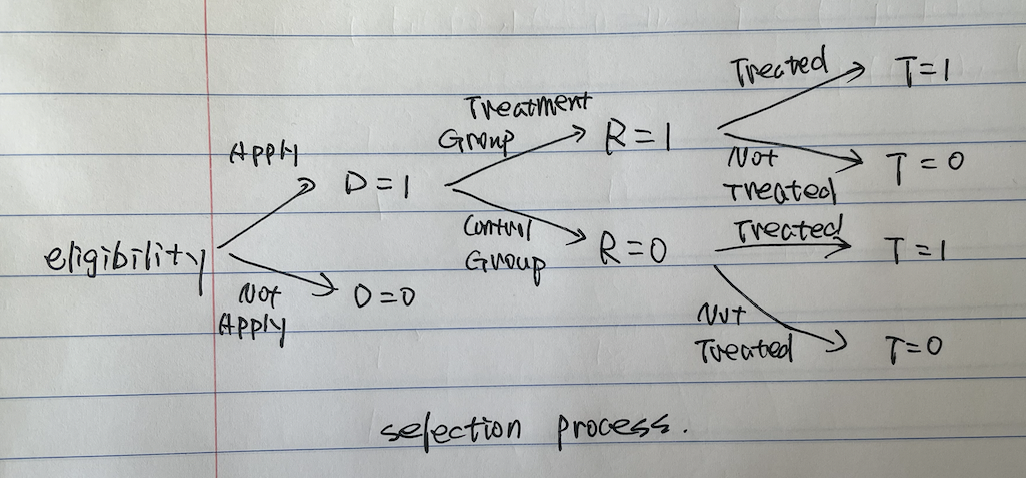
\includegraphics[scale=0.78]{Figures/applied_rct_selection}}
\caption{The Selection Process}\label{F:selection}
\end{figure}

First, the eligible units choose to apply or not. Then those applied units are randomly assigned to treatment and control groups. This is the world of \textit{non-perfect compliance}. Finally, we will have \textit{the treatment group no-shows}, that is, $D_{i} = 1, R_{i} = 1$ but $T_{i} = 0$, as well as \textit{the control group substitutions}, i.e., $D_{i} = 1, R_{i} = 0$ but $T_{i} = 1$. 

There is another complication, it is very likely that we will have \textit{the endogeneity problem}. That is, $\mathbb{E}(T, \epsilon) \ne 0$ or a stronger (but unnecessary) version $\mathbb{E}[\epsilon \mid T] \ne 0$. In this case, we consider the random variable $R$, which stands for random assignment, as an instrument random variable for $D$. We need to have $\operatorname{Cov}(R, D) \ne 0$ and $\mathbb{E}[R, \epsilon] = 0$ being satisfied for a legitimate instrument. The first condition is reasonable, since people will react to incentives. The second condition is guaranteed if we have random assignment.

\end{document}
